\section{Appendix A. UML charts}

\begin{figure}[h!]
\begin{center}
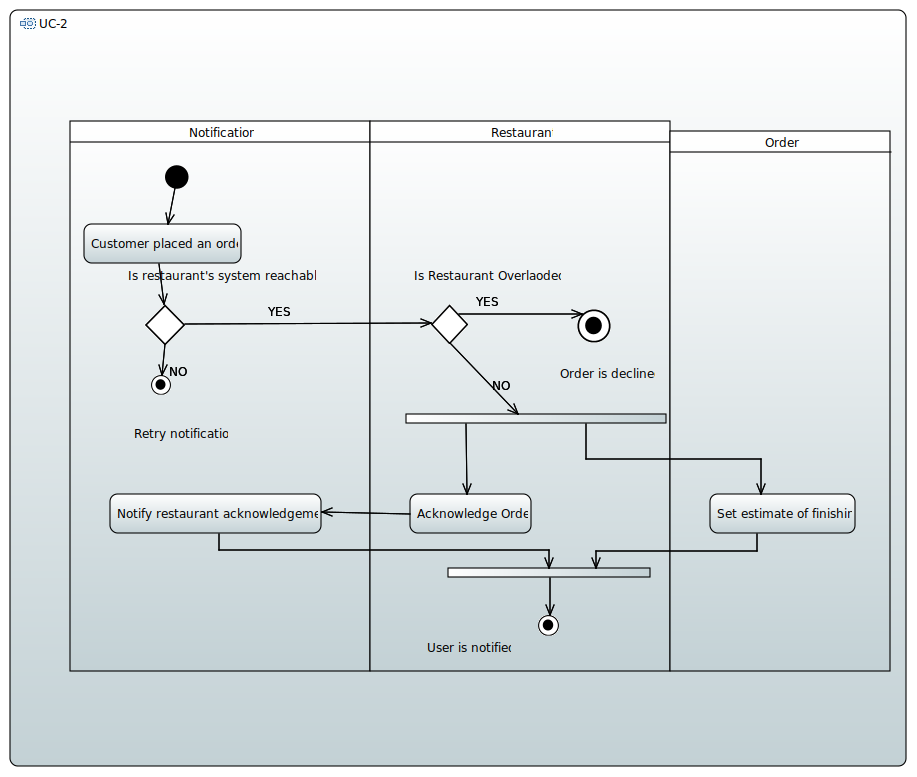
\includegraphics[scale=0.35]{FIGS/UC-2.PNG}
    \caption{Activity Diagram UC-2}
    \label{fig:act_diag2}
\end{center}
\end{figure}

\begin{figure}[h!]
\begin{center}
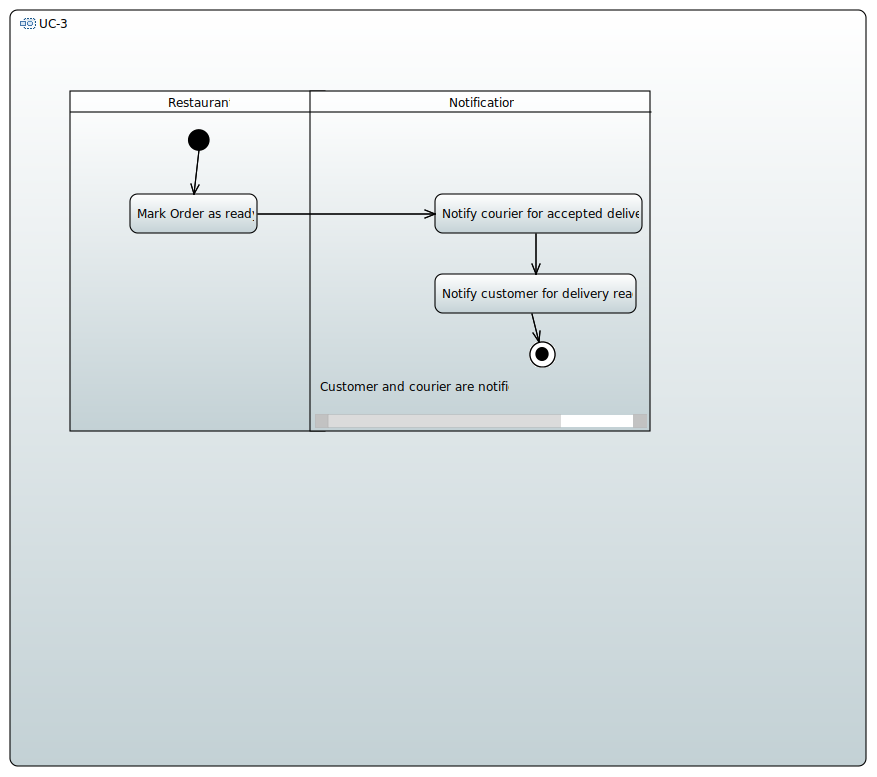
\includegraphics[scale=0.35]{FIGS/UC-3.PNG}
    \caption{Activity Diagram UC-3}
    \label{fig:act_diag3}
\end{center}
\end{figure}

\begin{figure}[h!]
\begin{center}
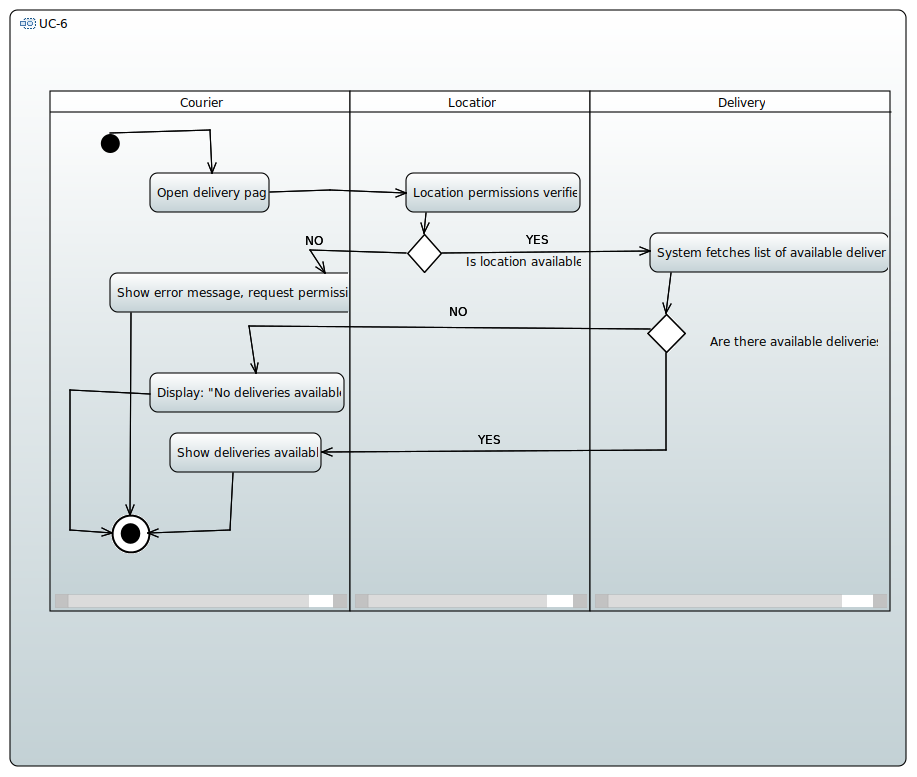
\includegraphics[scale=0.5]{FIGS/UC-6.jpg}
    \caption{Activity Diagram UC-6}
    \label{fig:act_diag2}
\end{center}
\end{figure}

\begin{figure}[h!]
\begin{center}
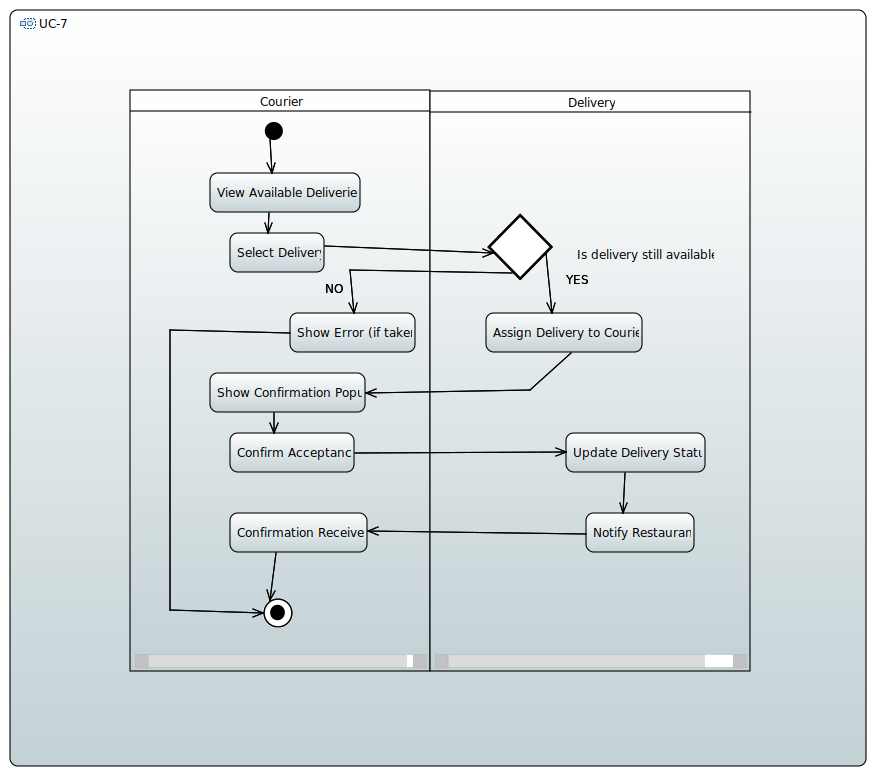
\includegraphics[scale=0.5]{FIGS/UC-7.jpg}
    \caption{Activity Diagram UC-7}
    \label{fig:act_diag3}
\end{center}
\end{figure}

\begin{figure}[h!]
\begin{center}
\includegraphics[scale=0.35]{FIGS/UC-21.PNG}
    \caption{Sequence Diagram UC-2}
    \label{fig:seq_diag3}
\end{center}
\end{figure}

\begin{figure}[h!]
\begin{center}
\includegraphics[scale=0.35]{FIGS/UC-31.PNG}
    \caption{Sequence Diagram UC-3}
    \label{fig:seq_diag3}
\end{center}
\end{figure}

\begin{figure}[h!]
\begin{center}
\includegraphics[scale=0.5]{FIGS/SD-UC-6.jpeg}
    \caption{Sequence Diagram UC-6}
    \label{fig:seq_diag3}
\end{center}
\end{figure}

\begin{figure}[h!]
\begin{center}
\includegraphics[scale=0.35]{FIGS/SD-UC-7.JPG}
    \caption{Sequence Diagram UC-7}
    \label{fig:seq_diag3}
\end{center}
\end{figure}

\begin{figure}[h!]
\begin{center}
\includegraphics[scale=0.35]{FIGS/UC-112.PNG}
    \caption{Sequence Diagram UC-11}
    \label{fig:seq_diag11}
\end{center}
\end{figure}